%% Beispiel-Präsentation mit LaTeX Beamer im KIT-Design
%% entsprechend den Gestaltungsrichtlinien vom Februar 2025
%%
%% Siehe https://sdq.kastel.kit.edu/wiki/Dokumentvorlagen

%% Beispiel-Präsentation
\documentclass[
                en,
                % kitgrid
                ]{sdqbeamer} 
 
%% Gruppenlogo, muss im Verezeichnis logos/ liegen
%% falls kein Gruppenlogo gewünscht, bitte \grouplogo{} aufrufen
\grouplogo{} 

%% Gruppenname und Breite (Standard: 89 mm)
\groupname{Institute for Physical Chemistry}
%\groupnamewidth{89mm}

% Beginn der Präsentation

\title[Ex. 3: Classification]{Maschinelles Lernen für die Chemie - Exercise 3}
\subtitle{Logistic Regression, Support Vector Machines}
\author[L. Pfeffer, M. Vogelbacher]{Leonie Pfeffer, Maike Vogelbacher}

\date[\today]{\today}

% Literatur 
 
\usepackage[citestyle=numeric,bibstyle=numeric,hyperref,backend=biber]{biblatex}
\addbibresource{presentation.bib}
\bibhang1em

\usepackage{lipsum}
\usepackage{ulem}
\usepackage{amsmath}
\DeclareMathOperator*{\argmax}{arg\,max}
\usepackage{tikz}
\usetikzlibrary{trees}

\begin{document}

%Titelseite
\begin{frame}[title blue vertical, picture=images/banner_2020_kit.jpg]
% \begin{frame}[title blue vertical, picture=images/palladio_bauplan]
	\titlepage
\end{frame}

\section{Logistic Regression}

\begin{frame}{Logistic Regression for Classification}
    \begin{greenblock}{Definition}
        \begin{itemize}
            \item Supervised learning
            \item Predict categorical outcomes
                \begin{itemize}
                    \item Binary classification: yes/no, 1/0
                    \item Multiple classes
                \end{itemize}
        \end{itemize}
    \end{greenblock}
    \begin{columns}
        \column{\kitthreecolumns}
        \begin{greenblock}{Goal}
            Predict the probability that a sample $x$ belongs to class 1
            \begin{equation*}
                P(y = 1 \mid x)
            \end{equation*}
            \begin{itemize}
                \item $x \in \mathbb{R}$: a single input feature
                \item $y \in \{0, 1\}$: target class label
            \end{itemize}
        \end{greenblock}

        \column{\kitthreecolumns}
        \begin{greenblock}{Decision Rule}
            Binary classification with decision boundary at $0.5$
            \begin{equation*}
                \hat{y} =
                \begin{cases}
                1 & \text{if } P(y = 1 \mid x) \geq 0.5 \\
                0 & \text{otherwise}
                \end{cases}
            \end{equation*}
        \end{greenblock}
    \end{columns}
\end{frame}

\begin{frame}{Sigmoid Function}
    \begin{columns}
        \column{\kitthreecolumns}
        \begin{greenblock}{a.k.a logistic function}
            \begin{equation*}
                P(y = 1 \mid x) = \frac{1}{1 + \exp[-(wx + b)]}
            \end{equation*}
            \begin{itemize}
                \item $w$: weight (slope)
                \item $b$: bias (intercept)
            \end{itemize}
        \end{greenblock}

        \column{\kitthreecolumns}
        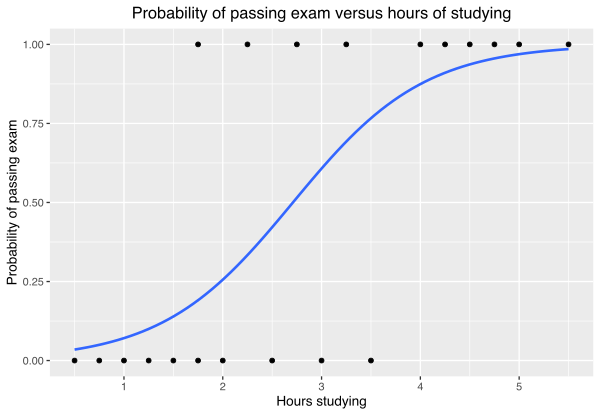
\includegraphics[width=\textwidth]{images/Exam_pass_logistic_curve.png}
    \end{columns}
\end{frame}

\begin{frame}{Multi-class Classification: Multinomial Regression}
    \begin{columns}
        \column{\kitthreecolumns}
        \begin{greenblock}{Example: Iris Dataset}
            \begin{itemize}
                \item $n = 150$ samples
                \item $d = 4$ features (sepal length/width, petal length/width)
                \item $K = 3$ classes (setosa, versicolor, virginica)
                \item $\boldsymbol{x}^{(i)} \in \mathbb{R}^2$ is the feature
                    vector for the $i^{th}$ sample
                \item $\boldsymbol{x}^{(i)} \in \{0, 1, 2\}$ is the class label
                    for the $i^{th}$ sample
            \end{itemize}
        \end{greenblock}

        \column{\kitthreecolumns}

        \begin{greenblock}{Multinomial Regression (softmax)}
            \textbf{Idea:} learn a single model with one set of weights per
            class, all weights are learned simultaneously
            \begin{equation*}
                P(y = k \mid \boldsymbol{x}) = \frac{\exp[-(\boldsymbol{w}_k^T
                \boldsymbol{x})]}{\sum_j \exp[-(\boldsymbol{w}_j^T
            \boldsymbol{x})]}
            \end{equation*}
            \begin{itemize}
                \item Weights: $W \in \mathbb{R}^{3 \times 4}$, where row $k$ is
                    $\boldsymbol{w}_k^T$
                \item Bias: $\boldsymbol{b} \in \mathbb{R}^3$
                \item $i \in \{1, ..., 150\}$
                \item Result: single vector of three class probabilities,
                    summing to 1
            \end{itemize}
        \end{greenblock}
    \end{columns}
\end{frame}

\begin{frame}{Multi-class Classification: One-vs-Rest}
    \begin{columns}
        \column{\kitthreecolumns}
        \begin{greenblock}{Example: Iris Dataset}
            \begin{itemize}
                \item $n = 150$ samples
                \item $d = 4$ features (sepal length/width, petal length/width)
                \item $K = 3$ classes (setosa, versicolor, virginica)
                \item $\boldsymbol{x}^{(i)} \in \mathbb{R}^2$ is the feature
                    vector for the $i^{th}$ sample
                \item $\boldsymbol{x}^{(i)} \in \{0, 1, 2\}$ is the class label
                    for the $i^{th}$ sample
            \end{itemize}
        \end{greenblock}

        \column{\kitthreecolumns}

        \begin{greenblock}{One-vs-Rest (sigmoid)}
            \textbf{Idea:} train $K$ separate binary classifiers, one for each
            class $k$, to distinguish class $k$ from all others
            \begin{equation*}
                P(y = k \mid \boldsymbol{x}^{(i)}) = \frac{1}{1 +
                \exp[-(\boldsymbol{w}_k^T \boldsymbol{x}^{(i)} + b_k)]}
            \end{equation*}

            \begin{itemize}
                \item Weights: $\boldsymbol{w}_k \in \mathbb{R}^4$
                \item Bias: $b_k \in \mathbb{R}$
                \item $i \in \{1, ..., 150\}$
                \item Result: three scalar probabilities per sample
            \end{itemize}
        \end{greenblock}
    \end{columns}
\end{frame}

\begin{frame}{Exercise: One-vs-Rest Regression}
    \begin{columns}
        \column{\kitthreecolumns}
        \begin{greenblock}{Training}
            \textbf{Create new labels}
            \begin{equation*}
                y^{(i)} =
                \begin{cases}
                1 & \text{if original class is}~k\\
                0 & \text{otherwise}
                \end{cases}
            \end{equation*}
            \textbf{Cross-entropy loss function}
            \begin{equation*}
                \mathcal{L}_k = - \sum_{i=1}^{n} \left[ y_k^{(i)}
                \log(\hat{y}_k^{(i)}) + (1-y_k^{(i)}) \log(1-\hat{y}_k^{(i)}) \right]
            \end{equation*}
            \begin{itemize}
                \item Typical for classification
                \item Can be optimized well due to global minimum
            \end{itemize}
        \end{greenblock}

        \column{\kitthreecolumns}
        \begin{greenblock}{Prediction}
            \textbf{Predictor for each class $k$}
            \begin{equation*}
                \hat{y}_k = \frac{1}{1 + \exp[-(\mathbf{w}_k^T \mathbf{x} +
                b_k)]}
            \end{equation*}
            \textbf{Select classifier with highest probability}
            \begin{equation*}
                \hat{y} = \argmax_k \hat{y}_k
            \end{equation*}
            
        \end{greenblock}
    \end{columns}
\end{frame}
% logistic function and its parameters
% example for 1D and nD -> multinomial logistic regression, OvR
% cross-entropy loss function


\section{Exercise}

\begin{frame}{Pandas Methods}
    \textbf{\texttt{pandas.DataFrame.value\_counts()}}
    \begin{itemize}
        \item Count the number of occurrences of each unique value in a
            DataFrame
    \end{itemize}
    \vfill
    \textbf{\texttt{pandas.DataFrame.info()}}
    \begin{itemize}
        \item Print summary of the DataFrame
        \item Similar to \texttt{pandas.DataFrame.describe()}
    \end{itemize}
    \vfill
    \textbf{\texttt{pandas.DataFrame.copy()}}
    \begin{itemize}
        \item Copy selected sub-DataFrames (e. g. columns) to a new DataFrame
            variable
        \item Changes in the copy will not influence the copy (default behavior)
    \end{itemize}
\end{frame}

\begin{frame}{Pair Plot}
    \begin{columns}
        \begin{column}{0.4\textwidth}
            \textbf{\texttt{sns.pairplot(DataFrame, hue="labels")}}
            \begin{itemize}
                \item Easy way to look at obvious correlations between different
                    features
            \end{itemize}
        \end{column}
        \begin{column}{0.6\textwidth}
            \centering
            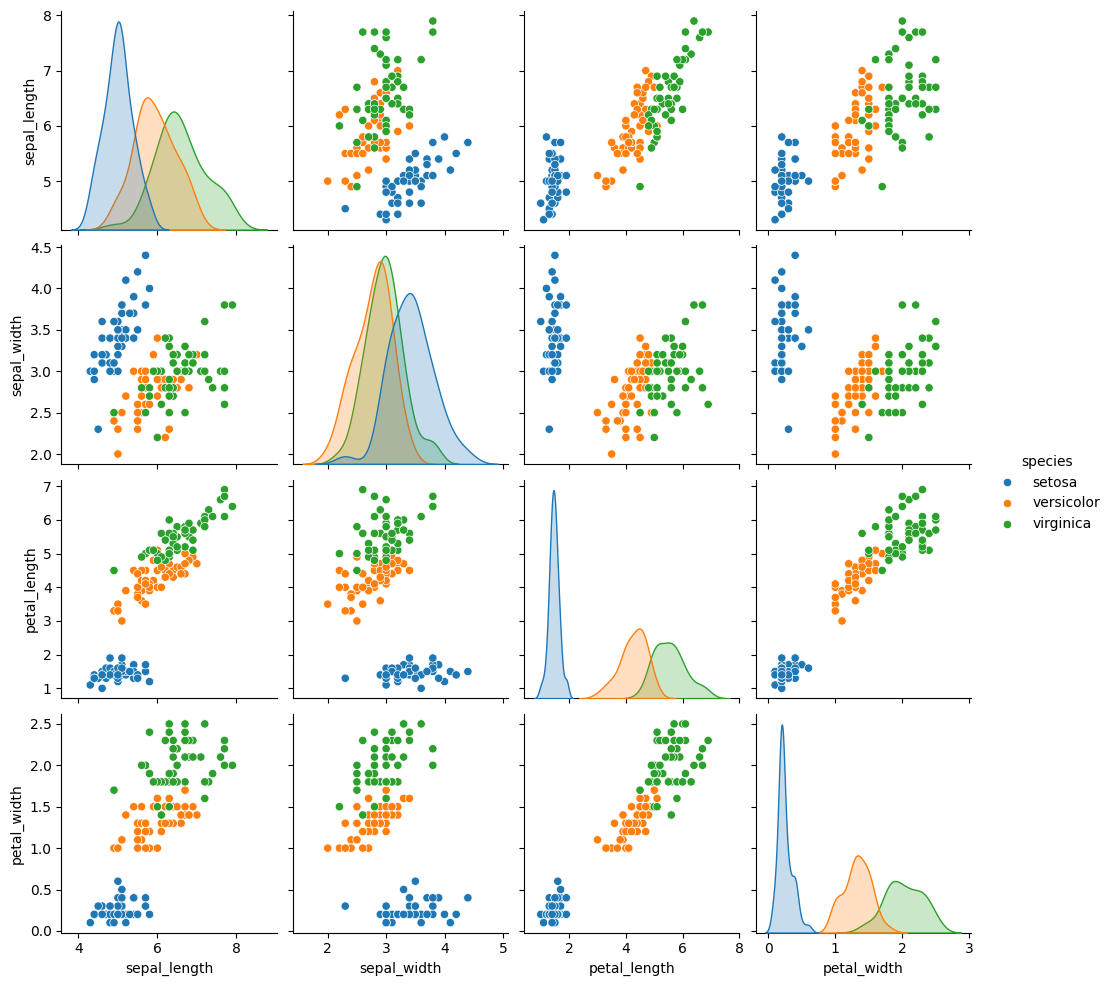
\includegraphics[width=0.8\textwidth]{./images/pairplot_iris.png}
        \end{column}
    \end{columns}
\end{frame}

\begin{frame}{Scaling Input Data}
    \textbf{Scikit-learn \texttt{StandardScaler}}
    \begin{itemize}
        \setlength\itemsep{2em}
        \item Scale data to a mean value of $\mu = 0$ and standard deviation of
            $\sigma = 1$
            \begin{equation*}
                x_\text{scaled} = \frac{x - \mu}{\sigma}
            \end{equation*}
        \item Create a StandardScaler instance: \\
            \texttt{scaler: StandardScaler = StandardScaler()}
        \item Compute the mean and standard deviation for each column for the
            scaling in the next step: \\
            \texttt{scaler.fit(training\_data)}
        \item Actual standardization: \\
            \texttt{training\_data\_scaled = scaler.transform(training\_data)}
    \end{itemize}
\end{frame}

\begin{frame}{Confusion Matrix}
    \textbf{\texttt{confusion\_matrix(y\_true, y\_predicted)}}

    \centering{}
    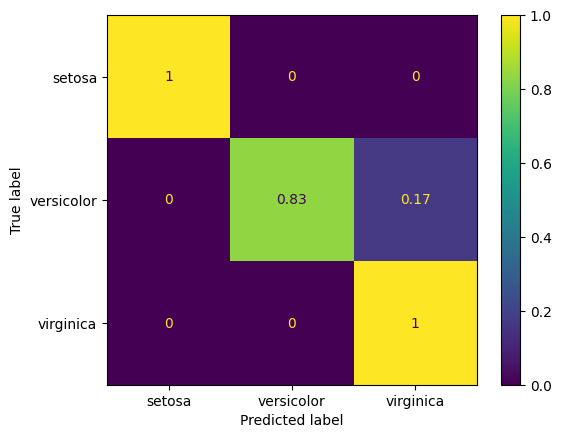
\includegraphics[width=0.5\textwidth]{./images/cm_iris.png}
\end{frame}

\appendix
% Slides here will not be counted in the page numbering nor will they
% appear in the navigation bar
\beginbackup

% \begin{frame}{Literature}
%     \begin{itemize}
%         \setlength\itemsep{2em}
%         \item Linear Regression~\nocite{Hastie-2009}
%             \printbibliography[keyword={hastie},title={Linear Regression}]
%         \item Bayes' theorem and probabilities~\nocite{wikipedia-bayes-en,
%             wikipedia-bayes-de}
%             \printbibliography[keyword={bayes}, title={Bayes' theorem and
%             probabilities}]
%     \end{itemize}
% \end{frame}

\backupend
\end{document}
